% This is samplepaper.tex, a sample chapter demonstrating the
% LLNCS macro package for Springer Computer Science proceedings;
% Version 2.20 of 2017/10/04
%
\documentclass[runningheads]{llncs}
%
\usepackage{graphicx}
\usepackage{lipsum}
\usepackage{makecell}
\usepackage{amsmath}
\usepackage{apacite}
\usepackage{bbm}
\usepackage{todonotes}
\usepackage{multirow}
\usepackage{caption}
\usepackage{subcaption}
\usepackage{booktabs}
% Used for displaying a sample figure. If possible, figure files should
% be included in EPS format.
%
% If you use the hyperref package, please uncomment the following line
% to display URLs in blue roman font according to Springer's eBook style:
% \renewcommand\UrlFont{\color{blue}\rmfamily}

\begin{document}
%
% \title{Master Research Project}
% \title{Multi-Horizon Forecasting with Extreme Gradient Boosting to enhance prediction accuracy of State-based Violence}
% \title{Multi-Horizon Extreme Gradient Boosting for Conflict Forecasting}
% \title{Conflict Forecasting with Uncertainty using Bagging and Multi-Horizon Extreme Gradient Boosting}
% \title{Probabilistic Conflict Forecasting using Multi-Horizon Natural Gradient Boosting}
    \title{Probabilistic Forecasting of Conflict-Related Fatalities - Natural Gradient Boosting}


%
%\titlerunning{Abbreviated paper title}
% If the paper title is too long for the running head, you can set
% an abbreviated paper title here
%
    \author{Oleksandr Zakotianskyi}
%
    \authorrunning{O. Zakotianskyi}
% First names are abbreviated in the running head.
% If there are more than two authors, 'et al.' is used.
%
    \institute{Vrije Universiteit Amsterdam, Netherlands\\
    \email{o.zakotianskyi@student.vu.nl}\\}
% \and
% CeDRI, Instituto Politécnico de Bragança, Portugal\\
% \email{author@ipb.pt}
% \and
% Instituto Politécnico do Cávado e do Ave, IPCA, Portugal\\
% \email{author@ipca.pt}}
%
    \maketitle              % typeset the header of the contribution
%
    \begin{abstract}
% The authors can submit a Short Paper or a Full Paper in English.
% The Short Paper must have between 2 and 3 pages.
% The Full Paper must have between 4 and 8 pages.

% The abstract should briefly summarize the contents of the paper in
% 15--250 words.
% Master Research Project Abstract

% Conflict research is increasingly influenced by modern computational and statistical techniques. Combined with recent advances in the collection and public availability of new data sources, this allows for more accurate forecasting models in ever more fine-grained spatial areas.

% For at least the last three decades, the international community has attempted to develop robust, accurate, and effective conflict early
% warning system for conflict prevention.

        Can we predict wars?
        How certain would we be in our predictions?
        This research presents the first publicly available and explainable early conflict forecasting model capable of
        forecasting conflict-related fatalities with uncertainty on a country-month level.
        The model seeks to be maximally transparent, uses publicly available data and produces predictions up to 14 months into the future.
        The performance demonstrated here indicates that the presented model can complement the field of conflict-warning
        systems and serve as a reference against which future improvements can be evaluated.

% Conflict research is increasingly influenced by modern computational and statistical techniques. Combined with recent advances in the collection and public availability of new data sources, this allows for more accurate forecasting models. For at least the last three decades, the international community has attempted to develop robust, accurate, and effective conflict early warning system. Current conflict modelling systems predict fatalities as a point estimate. Even thorough the interest in predicting fatalities as a probability distribution is growing, there are only few works reporting their estimates as probabilities.


% Recently, a second prediction competition was announced by the Peace and Research Institute of Oslo urging for global coverage models capable of predicting conflict-related fatalities with uncertainty. The goal of the competition is to forecast state-based violence for each of the next 12 months. This paper presents the probabilistic prediction of fatalities at a country-month level using the Natural Gradient Boosting. To facilitate accuracy a separate model for each predicted month is built, which results in surpassing the competition benchmark over all 4 years according to the main competition evaluation metric -  Continuous Ranked Probability Score (CRPS). The results demonstrate the feasibility of the approach and propose improvements to reduce the variance of predictions.

% This paper presents an approach capable of monthly fatalities prediction with uncertainty with global coverage for 3-15 months ahead.

% This paper presents an ensemble of models that improve over the prediction competition benchmark for predicting fatalities on a national level per month 12 months ahead for all countries.

% Natural gradient has been recently introduced to the field of boosting to enable the generic probabilistic prediction capability.


% an ensemble of models that improve over the prediction competition benchmark for predicting fatalities on a national level per month 12 months ahead for all countries.


% The final predictions improve over the prediction competition benchmark for predicting fatalities on a national level per month.

% The accuracy is improved by multi-horizon ensemble learning. The variance to each estimation per month is added by bootstrap aggregation which allows for models that are more sensitive to changes in conflict dynamics. The results demonstrate the feasibility of the approach and set a new benchmark for my further studies of the conflict research field.

% The results demonstrate the potential of the approach and set a path toward effective global conflict early warning systems.

% Importance of interstate conflict prediction
% ViEWS competition
% This paper presents initial work that outperforms both competition benchmarks and sets a path toward a complex conflict prediction model.


% Thesis abstract
% Papers to use as inspiration for writing:
% ViEWS Havard 2019


        \keywords{Interstate conflict modelling \and Early Conflict Warning System \and Fatalities prediction \and Predicting with uncertainty}
    \end{abstract}
%
%
%


    \section{Introduction}
% \begin{itemize}
%     \item Conflict research
%     \item The goal of such models and who are their stakeholders
%     \item Uncertainty estimation
%     \item Importance of explainability
%     \item Two types of models: country level and PRIO grid level
%     \item Previous work was focused on predicting the probability and fatalities from civil wars only as this is easier to model
%     \item New datasets allow for enhanced models
%     \item The dataset I used is from the PRIO competition. They also publish two benchmarks for this competition. There are two benchmarks: Last Historical Poisson and Benchmark Boostrap. Explain what they use.
%     \item This work uses NGBoost. Some intro about NGBoost. Benefits of NGboost - prob forecasting and explainability. It has comparative accuracy to XGBoost.
%     \item Accuracy of the model: it beats 3/4 years of benchmark
% \end{itemize}

% Motivation
    A new wave of violent conflicts around the world raises concerns about the security of the whole world. According to the ACLED Conflict Index 12\% more conflict occurred in 2023 compared to 2022, and the amount of conflict increased by 40\% compared to 2020. An underlying assumption and motivation of conflict early warning systems is that enhanced prediction and forecasting can better inform decision-making, reduce risk, and trigger more robust prevention and response measures from international actors. Policymakers are interested in uncovering the conflict dynamics and making robust forecasts to take anticipatory actions and reduce the impact on vulnerable people. At the same time, regular citizens are looking for accurate and not biased forecasts for their own security and awareness.


% Typically, stakeholders of Early Conflict Warning Systems are interested in the most likely outcome (a point prediction), but also in the lower-probability risk that conflicts escalate catastrophically (the tail ends of the probability distribution). Stakeholders are also interested in knowing how uncertain the forecasts are. Setting the communication challenges aside for this context, predictions of war intensity as probability distributions come closer to what user groups need than point estimates or simple dichotomous classification models.

% What is the problem and how do you want to solve it?
% Beginning with the landmark studies of Collier and Hoeffler (1998, 2004), a quantitative turn in conflict research led to a surge of publications studying quantitative risk factors affecting the conflict propensity of regions and states (Fearon and Laitin 2003; Hegre and Sambanis 2006)

    A decade ago inspiring studies of Hedge 2013 and Chadefaux 2014 marked a path towards a new generation of models - production-ready Early Conflict Warning Systems. By now at least a couple of dozen Early Conflict Warning Systems are deployed and to some degree are used for decision-making (Rod with Hegre 2022 and Muggah 2022). Great progress in this development was thanks to the first prediction competition organized by the ViEWS team in 2020, with the main focus to increase the accuracy of the state-of-the-art conflict prediction models. When the improved models were deployed and feedback from stakeholders was gathered, it became apparent that additional improvements were needed. According to the feedback, the stakeholders are interested not only in the most likely outcome (a point prediction), but also in the lower-probability risk that conflicts escalate catastrophically (the tail ends of the probability distribution), and understanding how uncertain the forecasts at hand are. These preferences urge for a new generation of forecasting models that present their estimates as probability distributions.


% Since then the ViEWS model has improved and till today the production version of it uses


% Such developments allowed for gathering feedback from stakeholders.

    % Multiple conflict forecasting models were built and deployed in the last decade and the stakeholders' feedback was gathered. are interested in forecasts that would . To close this gap, t


% The majority of such systems are private, only a couple publish their forecasts publicly and even fewer explain their data inputs and open source their codebase.


% Research teams worldwide are focused on increasing the accuracy of the existing Early Conflict Warning Systems and deploying pipelines that allow for frequent updates. As some of the models were already deployed, and feedback from stakeholders was gathered, it became apparent that additional improvements are needed. According to the feedback, the stakeholders are interested not only in the most likely outcome (a point prediction), but also in the lower-probability risk that conflicts escalate catastrophically (the tail ends of the probability distribution), and understanding how uncertain the forecasts at hand are. These preferences urge for a new generation of forecasting models that present their estimates and perform predictions of war intensity as probability distributions.


% come closer to what user groups need than point estimates or simple dichotomous classification models.

% There are three types of conflict prediction models – classification, conflict risk prediction, and continuous fatalities prediction.

% Research teams worldwide are putting great effort into developing different prototypes
% of predictor frameworks that can correctly and timely forecast conflict escalation in the
% future based on the economic, political, demographic and social data available today in
% individual states and regions.


% The great examples of such systems are ViEWS and Conflict Forecast and others. In their current implementation, these models are


% ...
% Subsequent paragraphs highlight your contributions.
% and use forward references to the next sections
% \section{Main contributions}
    In an attempt to close this gap, the ViEWS team has announced the second prediction competition, now focusing on predicting the distribution of conflict-related fatalities instead of simple point forecasts. As a response, I present the open-source model for forecasting fatalities with uncertainty. The model builds upon the Natural Gradient Boosting framework by Duan et. al. \cite{duan2020ngboost} which allows for estimating conditional probability distribution for each separate prediction. The overall accuracy of the model is on par with traditional gradient boosting techniques, which allows for improvement over the competition benchmark for 3 out of 4 prediction years.


    \section{Summary of contributions}
    \begin{enumerate}
        \item I present a model for forecasting conflict-related fatalities based on the Natural Gradient Boosting framework (Section \ref{section_ngboost} and results in Section \ref{section_results}).
        \item I clean and improve the competition dataset by removing rows with too many missing values and adding new dimensions of data, which results in increased performance (Section \ref{section_input_data}).
    \end{enumerate}


    \section{Methodology}
    To address the forecasting task, I divide the model development into smaller sub-tasks and detail each in this section. I describe the original input data, how it was processed and how the model was trained and fine-tuned.

    \subsection{Level of analysis and prediction window}
    \label{method_pred_wind}
    The model generates forecasts at the country-month level of analysis. The cm level is useful for predictions of new conflicts where no known actors exist, and to model processes at the government level. The set of countries is defined as in \cite{GleditschWard}, and the geographical extent of countries by CShapes (Weidmann, Kuse \& Gleditsch, 2010).

    The model makes predictions for all months from January to December of the next year based on the data till October of the previous year. For instance, to predict monthly predictions for 2024, the inputs are strictly until October 2023 inclusive. I use 'One step ahead' modelling with 12 months in the test set, which as a result produces forecasts for 12 months for each country. As the last available month with data is October, the dependent variable is shifted by 14, s.t. if the model produces forecasts for the whole year of 2024, the test set spans from November 2022 to October 2023, and the train set includes every month until October 2022 inclusive.

    \subsection{Input Dataset}
    \label{section_input_data}
    I use the dataset published by the ViEWS team for the second prediction competition \cite{predictionchallenge2023}. The published dataset merges multiple open-source datasets, with the most important data being on amounts of fatalities with spatial and temporal features from the UCDP Georeferenced Events Dataset, the World Development Indicators (World Bank, 2015), data on politically excluded ethnic groups (Cederman, Wimmer \& Min, 2010), demographic factors (Lutz et al., 2007), protests from ACLED (Raleigh et al., 2010), and data on institutions from V-Dem (Coppedge et al., 2011), and data on national water resources from AQUASTAT (AQUASTAT Glossary, FAO, 2019). The dataset is a great work by the ViEWS team. It covers 382 months from 1990 to 2023 for 213 unique country IDs (defined according to the Gleditsch \& Ward system) and comprises 128 columns.

    As for the dependent variable, I follow the ViEWS competition guidelines and choose state-based conflict (`sb`). The other options for the dependent variable according to the definition by Melander, Pettersson \& Themner (2016) are one-sided violence against civilians (`os`), and nonstate conflict (`ns`). Cases of `os` and `ns` are less numerous and were studied less extensively. Additionally, a large share of these events are also outcomes of state-based conflicts: much of the violence against civilians is perpetrated by governments and rebel groups to weaken opponents, and much non-state conflict is infighting between rebel groups that also conflict with the government. I keep `os` and `ns` conflicts in the dataset as independent variables.


    \begin{figure}[htbp]
        \centering

        % First subfigure
        \begin{subfigure}[b]{0.49\textwidth}
            \centering
            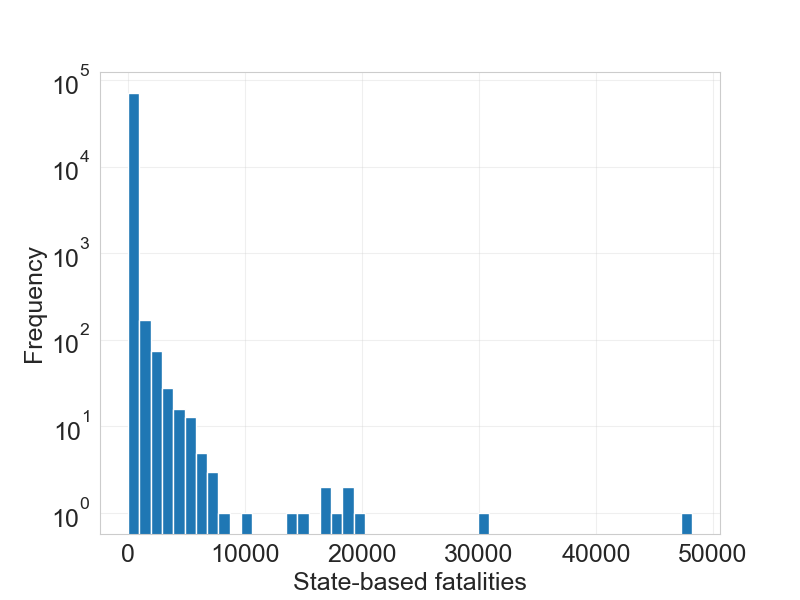
\includegraphics[width=\textwidth]{Figures/ged_sb_distribution.png}
            \caption{Distributions of 'sb' fatalities}
            \label{fig:histogram_ged_sb}
        \end{subfigure}
        \hfill
        % Second subfigure
        \begin{subfigure}[b]{0.49\textwidth}
            \centering
            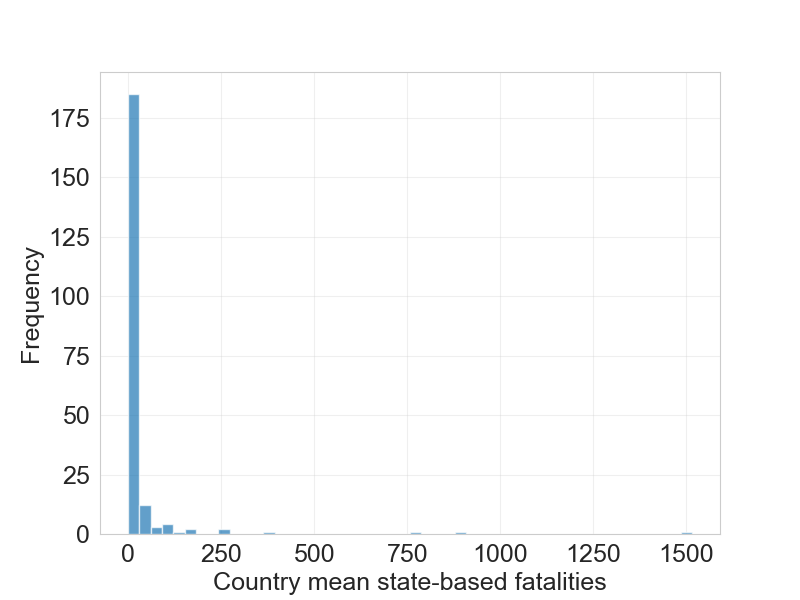
\includegraphics[width=\textwidth]{Figures/per_country_mean_ged_sb_distribution.png}
            \caption{Distribution of country mean 'sb' fatalities}
            \label{fig:histogram_mean_ged_sb}
        \end{subfigure}

        \caption{Distribution of fatalities with and without per country aggregation. The dependent variable is highly skewed to the right with Skewness=71 and Kurtosis=7810}
        \label{fig:dist_fatalities}
    \end{figure}


    The distribution of the state-based 'sb' fatalities is shown in Figure \ref{fig:histogram_ged_sb} and the distribution of the mean fatalities per country is shown in Figure \ref{fig:histogram_mean_ged_sb}. The dependent variable is highly skewed to the right and has a long tail on the right side.

    Moreover, some variables are highly correlated. The high correlation of $|0.75|$ occurs for 78 out of 125 numeric variables, mostly for features from VDEM, WDI datasets and some spatial decays. The full correlation matrix is shown in the Appendix section \ref{sec:corr_mat}.


% \todo{Give an overview of the data. Skewness of the dependent variable (its distribution), some statistics on the number of countries that never had violence in their all history}
% \todo{add correlation matrix of the dataset}
% \todo{Make everything below a separate section}

    \subsection{Dataset Processing}
    In this section, I clean the original ViEWS dataset, create a dependent variable for the prediction task and populate additional data to the dataset.

    \subsubsection{Removal of some countries}
    I find several problems with the original dataset, namely:
    \begin{itemize}
        \item There are cases where the same country has multiple country IDs in the same month and some variables for one of the instances are not populated.
        \item There are countries where almost all variables except for the dependent variable are 0, or even the dependent variable is also 0. This usually happens for low-populated islands, micro-states or countries which do not exist now and lack reliable data.
    \end{itemize}



    To address these issues I calculate the percentage of zero values for each of the country-month and also the mean per country. To account for the fact that some features are spatial or temporal lags of the other I exclude from the analysis all spacial and temporal lag features. Additionally, as previous violence is a good prediction of future violence and the model should be able to learn not only fluctuations of the dependent variable but also infer future violence from the country's indexes, I exclude from the analysis all features that are related to fatalities ('sb', 'ns' and 'os' violence and ACLED data on protests). After the column exclusions, 89 data columns are left for analysis.


    The percentage of missing values per country is defined as an average proportion of zero values in a given subset of columns for this country:
    \todo{Adjust indicator function to the format in the CRPS}
    \[
        \text{Country mean percentage of zero values} = \left( \frac{\sum_{m=1}^{M} \left( \frac{\sum_{i=1}^{N} Z_{im}}{N} \right)}{M} \right) \times 100
    \]

% \[
% Z_{ij} = \begin{cases}
% 1 & \text{if the value in column } i \text{ of row } j \text{ equals 0} \\
% 0 & \text{otherwise}
% \end{cases}
% \]
    where

% \[
% Z_{ij} = \begin{cases}
% 1 & \text{if the value in column } i \text{ of row } j \text{ equals 0} \\
% 0 & \text{otherwise}
% \end{cases}
% \]

    \begin{itemize}
        \item \( N \) is the total number of columns to analyse.
        \item \( M \) is the total number of months per country ID.
        \item \( Z_{im} \) is the indicator function for the \(i\)-th column in the \(m\)-th row (country-month), defined as:
        \[
            Z_{ij} = \begin{cases}
                         1 & \text{if the value in column } i \text{ of row } m \text{ equals 0} \\
                         0 & \text{otherwise}
            \end{cases}
        \]
    \end{itemize}


    With the percentage of missing values calculated, the dataset is processed in two steps:

    \begin{enumerate}
        \item \textbf{Correlates-of-War mapping}: An alternative to Gleditsch\&Ward State System Membership exists and was published by the Correlates of War (CoW) project. The major difference between these systems is that CoW does not include states with populations lower than 250,000, which automatically excludes all microstates. Microstates are insignificant actors in a geopolitical landscape for which data collection is usually not done properly and major datasets do not consider these countries. By manual inspection, I found that all states from the original dataset that cannot be mapped to the CoW system are all microstates, with more than 70\% of missing values. Thus, these countries are dropped from the dataset.
        \item \textbf{Dropping countries with more than 20\% of zero values}: Many studies find that the previous violence is a good predictor of future violence\todo{cite}. Thus, keeping countries with only populated fatality variables with their spatial and temporal lags and the majority of other structural variables being 0 would only incentivise the model to ignore the country indexes and focus on learning patterns of previous violence. To minimise the chances of such learning, I drop all countries which have a percentage of missing values of more than 20\%. The calculation results of the mean missing values per country are presented in Table \ref{tab:missing_values}. One can see that the majority of countries with a mean zero values percentage of more than 20\% are either microstates or short-lived countries or countries for which data collection was not reliable.
    \end{enumerate}

    \begin{table}[h]
        \centering
        \begin{tabular}{|r|l|r|l|l|r|}
            \hline
            \makecell{Country \\ ID} & \makecell{Country name}             & \makecell{Percentage of \\ missing values (\%)} & \makecell{Min      \\ date} & \makecell{Max                     \\ date} & \makecell{Max                 \\ fatalities} \\ \hline
            187.000 & Czechoslovakia      & 100.00 & 1990-01 & 1992-12 & 0     \\ \hline
            189.000 & Russia (Soviet Union)      & 100.00 & 1990-01 & 1991-08 & 144     \\ \hline
            232.000 & Kosovo      & 100.00 & 2008-03 & 2021-10 & 0     \\ \hline
            247.000 & Yugoslavia      & 100.00 & 1991-11 & 1992-04 & 1284     \\ \hline
            248.000 & Russia (Soviet Union)                 & 100.00  & 1991-08 & 1991-08 & 0   \\ \hline
            250.000 & Russia (Soviet Union)                 & 100.00  & 1991-09 & 1991-09 & 0   \\ \hline
            252.000 & Russia (Soviet Union)                    & 100.00  & 1991-10 & 1991-10 & 0     \\ \hline
            253.000 & Russia (Soviet Union)                     & 100.00  & 1991-11 & 1991-11 & 1     \\ \hline
            254.000 & Russia (Soviet Union)                     & 100.00  & 1991-12 & 1991-12 & 0     \\ \hline
            188.000 & Yugoslavia & 98.88  & 1990-01 & 1991-11 & 351     \\ \hline
            227.000 & Yugoslavia   & 97.75  & 1992-04 & 2006-06 & 560     \\ \hline
            26.0000 & Bahamas                     & 70.85  & 1990-01 & 2021-10 & 0     \\ \hline
            140.000 & Brunei       & 60.67  & 1990-01 & 2021-10 & 0     \\ \hline
            27.0000 & Belize    & 58.80  & 1990-01 & 2021-10 & 0     \\ \hline
            186.000 & German Democratic Republic               & 49.44  & 1990-01 & 1990-10 & 0     \\ \hline
            197.000 & Yemen, People's Republic                     & 49.44  & 1990-01 & 1990-05 & 0     \\ \hline
            198.000 & Taiwan                   & 44.20  & 1990-01 & 2021-10 & 0 \\ \hline
            196.000 & Yemen, Arab Republic            & 25.84  & 1990-01 & 1990-05 & 0     \\ \hline
            185.000 & German Federal Republic         & 24.72  & 1990-01 & 1990-10 & 1  \\ \hline
            192.000    & South Africa                       & 19.10   & 1990-01    & 1990-03    & 0  \\ \hline
            230.000    & Serbia                       & 17.98   & 2006-06    & 2008-02    & 0  \\ \hline
            191.000    & Ethiopia                       & 14.14   & 1990-01    & 1993-05    & 16545  \\ \hline
            180.000    & Solomon Islands                       & 13.48   & 1990-01    & 2021-10    & 2  \\ \hline
            83.0000    & Bosnia-Herzegovina                       & 10.71   & 1992-04    & 2021-10    & 4423  \\ \hline
            ....    & ....                       & ....   & ....    & ....    & ....  \\ \hline
        \end{tabular}
        \caption{Mean percentage of missing values for Gleditsch-Ward Country IDs in the original dataset after dropping countries that could not be mapped to the CoW state membership system}
        \label{tab:missing_values}
    \end{table}

% The model cannot infer fluctuations if too many values are zero and will simply rely on previous violence, which is not good.

    The resulting dataset comprises 177 or 169 unique country IDs depending on whether the Gleditsch\&Ward or CoW state membership systems are used. This difference comes from the fact that for some states that experienced revolutions and changes in government structure (e.g. Sudan in July 2011, Indonesia in May 2002 or multiple instances of Russia in 1991), the Gleditsch\&Ward system defines a different country ID, while CoW keeps the same.

    As the last step, the country IDs are encoded using OneHotEncoder according to the Gleditsch\&Ward system.

    \subsubsection{Dependent variable shifting}
    As explained in Section \ref{method_pred_wind}, the dependent variable is generated by shifting the state-based fatalities column by 14 months back to create a dependency suitable for forecasting. Because the Gleditsch\&Ward country membership system changes country ID every time the government structure changes, the dependent variable is shifted based on CoW country ID, which does not change in such cases. As ViEWS competition suggests, the country-months dataset is merged with country-month 'actuals' for the predicted year, which creates an expected 2-month gap between the test set and the predicted year and as a result a gap between the train set and the test set. The visualization of the split is provided in Figure \ref{train_test_split}.

    \begin{figure}[h]
        \includegraphics[width=0.9\textwidth]{Figures/train test thesis png.png}
        \centering
        \caption{Train and Test datasets for 2022 prediction year. The test set spans 12 months and each month in the test set predicts 14 months ahead}
        \label{train_test_split}
    \end{figure}

    \subsubsection{Regions addition}
    \todo{Regions addition}
    According to multiple studies in the peace research community, adding a region component to the dataset helps in increased accuracy or explaining variability in modelling conflict \todo{cite}. The intuition behind this finding is that different regions have different determinants influencing conflict and propensities for instability. Goldstone in his early research notes five regions that account for similar “regional and temporal distributions” in both the control and problem datasets [9].
% Goldstone finds that modelling by region rather than globally increases model accuracy.

    Shortly after, researcher Hegre demonstrated a modelling approach that included
    regions as predictor variables. Hegre defined nine regions revised from the United Nations’ regional definitions. He posited that the region variable improves the quality of predictions by maximizing the explained variance in the dataset, but questioned the duration of this assistance for forecasts more than a decade forecasting horizon as the heterogeneity of the region might change over time[16].

    To incorporate the regional dynamic, I add two categorical variables: seven global and 23 smaller regions according to World Bank Development Indicators. These categorical variables are encoded using OneHotEncoder and added to the dataset.

    \todo{cite Goldstone9 , Hegre16 Neumann 21 from page 100 US dissertation}

    \subsubsection{Least Important Features Drop}
    After the country IDs and regions are encoded the number of dimensions in the resulting dataset explodes, which may lead to the model's underperformance. To define the least important features, I run XGBoost regressor for a particular configuration of the dataset and the least important features are dropped before the main algorithm is run.

    \todo{Drop 35 least important features}

    \subsubsection{Parametrization}
    The parametrisation for the dataset preprocessing is used to test different hypotheses about the data and allow for flexibility. The list of fine-tuned parameters that support fine-tuning and concern data preprocessing is shown in Table \ref{tab:finetune-par} under the 'Data processing parameters' category.

% I argue that having a global model that takes into account every small state is beneficial, but then the quality of data for each predicted country must be in place. Microstates are insignificant actors in a geopolitical landscape for which data collection is usually not done properly and major datasets do not consider these countries. An alternative to Gleditsch\&Ward State System Membership exists and was published by the Correlates of War (CoW) project. The major difference between these systems is that CoW does not include states with populations lower than 250,000, which automatically excludes all microstates. By manual inspection, I found that all states from the original dataset that cannot be mapped to the CoW system are all microstates, with more than 70\% missing values. Thus, these countries are dropped from the dataset.


% The resulting dataset

% \todo{table of dropped country IDs and reason for dropping them}
% \todo{How I prepare data}
% \todo{Remove small islands and countries that have more than 25 of 0 values within descriptors in the dataset}
% \todo{What is the resulted dataset}
% How I prepare data
% I find that some countries have multiple zero values
% Remove small islands and countries that have more than 25% of 0 values within descriptors in the dataset
% Add regions
%

    \subsection{Natural Gradient Boosting}
    \label{section_ngboost}
    Gradient boosting (Friedman, 2001) is a supervised learning technique where several weak learners (or base learners) are combined in an additive ensemble. The model is learnt sequentially, where the next base learner is fit against the training objective residual of the current ensemble. The output of the fitted base learner is then scaled by a learning rate and added to the ensemble.

    Natural gradient boosting NGBoost\cite{duan2020ngboost} is a framework for probabilistic prediction with competitive state-of-the-art performance on a variety of datasets. NGBoost combines a multi-parameter boosting algorithm with the natural gradient to efficiently estimate how parameters of the presumed outcome distribution vary with the observed features. NGBoost can be used with any base learner, any family of distributions with continuous parameters, and any scoring rule. Duan et al. admit that point prediction will always be best with a dedicated model for that purpose, but they find the loss in RMSE is not substantial if NGBoost is used to support probabilistic regression.

    \todo{I test two distributions: Natural and Poisson, cite a website for distributions}
    While NGBoost supports multiple distributions \cite{NGBoost_dist}, in this work two distributions are tested: Natural and Poisson. The Poisson distribution, which is a discrete probability distribution, models the dependent variable as a whole number, which is ideal for predicting fatalities. On the other hand, the Natural distribution predicts the dependent variable as a real number, which can be negative. Moreover, the decent part of the predicted distribution can be negative if the prediction is around 0 but the variance is high. This requires additional handling, as otherwise predictions do not make sense.

    The problem of negative predictions for a feature that was non-negative throughout the whole train set with regression models is common. The gradient-boosting regression methods are unaware of feature boundaries and operate by splitting the tree based on whether the value is higher or lower\todo{cite and rephase}. While with point prediction the negative values of fatalities are simply converted to 0, in the case of distributions the handling of negative values in the distribution is dubious. ViEWS competition specifies default handling for negative predictions as clipping them to 0, which creates a bias towards 0 value, greatly changing the predicted distribution and impacting the CRPS and Mean Interval Score. I choose to resample the predicted distribution removing negative values. The processing of predictions is done in two steps:
    \begin{enumerate}
        \item The model outputs 1000 predictions for each country-month in the test set.
        \item All predictions are converted to integers.
        \item In case some country-month predictions have negative values, these are removed from the prediction set and the non-negative values are randomly resampled to fill in the created gaps.
    \end{enumerate}

    The difference between clipping the negative predictions to 0 and resampling is shown in Figure \ref{fig:dist_comp}. When resampling the mean of the predicted distribution is shifted towards a higher value of fatalities, but on the other hand, it does not place a disproportionate amount of confidence in the 0 value as clipping does. In Figure \ref{fig:histograms_Afghanistan}, the model under-predicted fatalities, and resampling shifted the mean further which benefited the CRPS metric; in Figure \ref{fig:histograms_Pakistan}, the model over-predicted fatalities and clipping predictions to 0 benefited the CRPS metric.

    \begin{figure}[htbp]
        \centering

        % First subfigure
        \begin{subfigure}[b]{\textwidth}
            \centering
            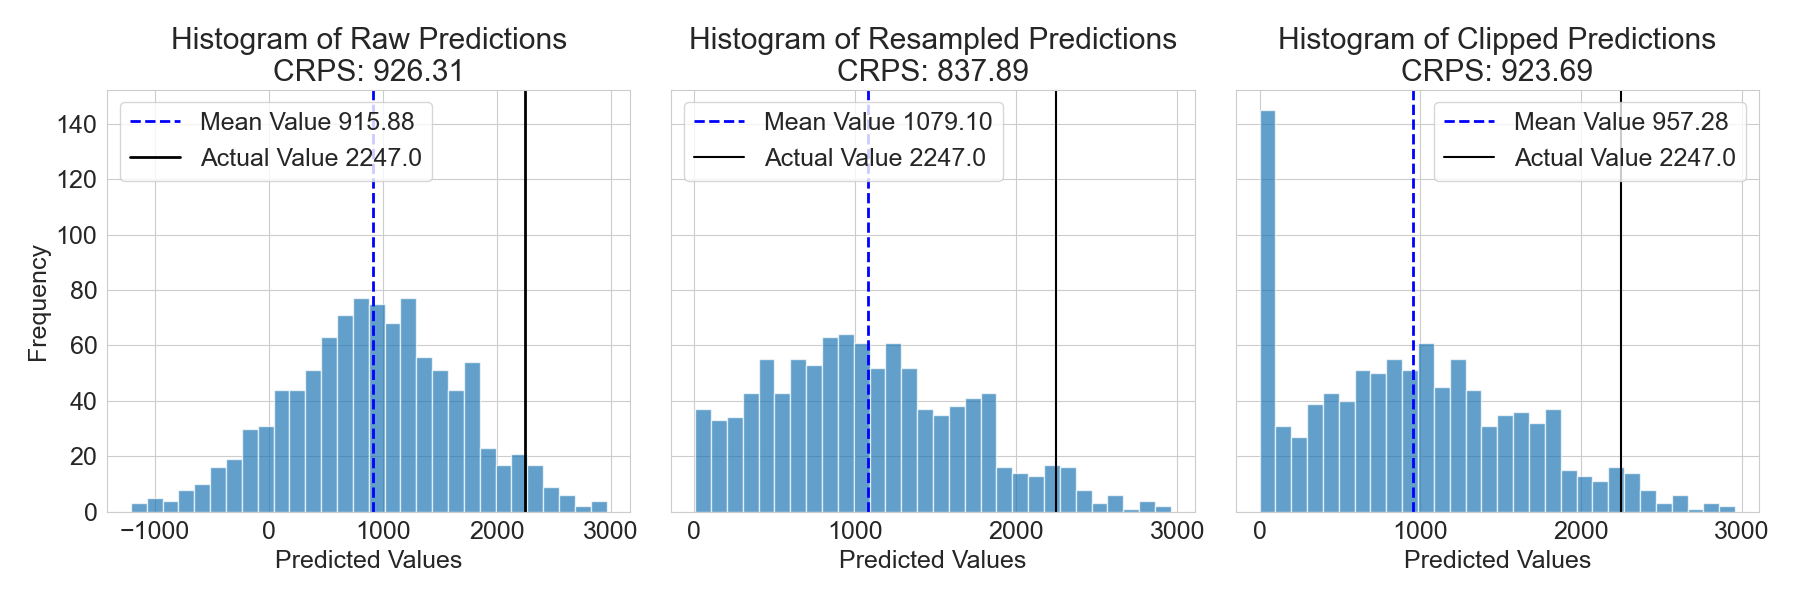
\includegraphics[width=0.8\textwidth]{Figures/histograms_Afghanistan_2020-11.png}
            \caption{Prediction distributions for Afghanistan November 2020 (month\_id: 477)}
            \label{fig:histograms_Afghanistan}
        \end{subfigure}

        \vspace{1em} % Adjust the vertical space between the subfigures as needed

        % Second subfigure
        \begin{subfigure}[b]{\textwidth}
            \centering
            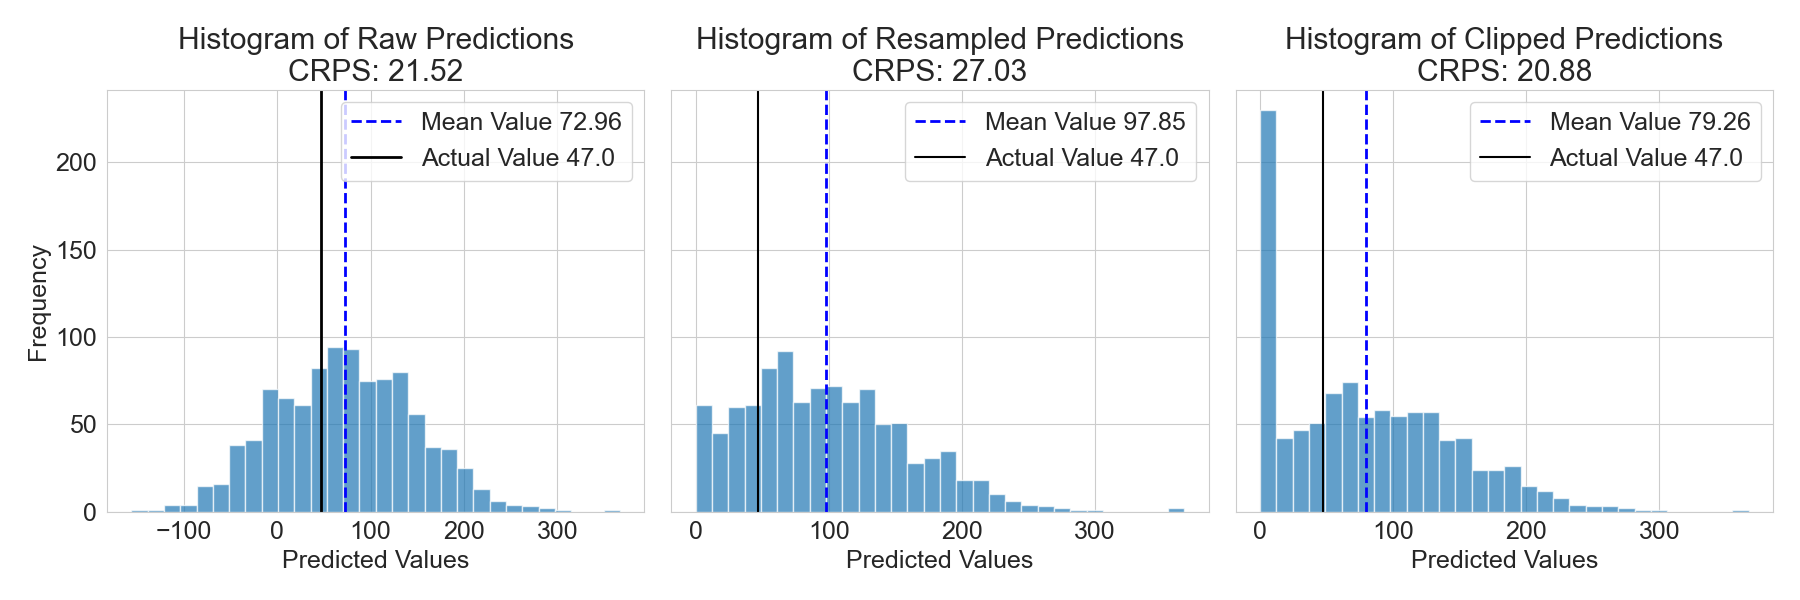
\includegraphics[width=0.8\textwidth]{Figures/histograms_Pakistan_2020-07.png} % Replace with the second image filename
            \caption{Prediction distributions for Pakistan July 2020 (month\_id: 473)}
            \label{fig:histograms_Pakistan}
        \end{subfigure}

        \caption{Comparison of raw, resampled and clipped fatalities distributions with negative tails for two county-month cases. }
        \label{fig:dist_comp}
    \end{figure}


% Not to change the form of distribution, I remove all the na

% \todo{maybe compare a figure side by side showing a prediction with big tails}

% \textbf{Evaluating results:} By nature, the number of fatalities cannot be negative. However,

    \subsection{Scoring Criteria}
    I adhere to the main evaluation metric of the ViEWS competition - the Continuous Ranked Probability Score (CRPS). The competition also defines two additional metrics that complement the CRPS: Ignorance score and Mean Interval Scores. I also report those metrics for comparability with other submissions of the competition.

    \subsubsection{Continuous Ranked Probability Score (CRPS)}

    The CRPS is a scoring function that compares a single ground-truth value to its predicted distribution. This property makes it relevant to Bayesian machine learning, where models usually output distributional predictions rather than point-wise estimates. The CRPS is defined as follows:

    The continuous rank probability score is defined as:


    \begin{equation}
        CRPS(F,y) = \int_{\mathbb{R}} (F(x) - \mathbbm{1}(x - y))^2 \, dx
    \end{equation}

    where \(\mathbbm{1}(z)\) is the indicator function (or Heaviside step function), defined as

    \begin{equation}
        \mathbbm{1}(z) =
        \begin{cases}
            1 & \text{if } z \geq 0 \\
            0 & \text{otherwise}
        \end{cases}
    \end{equation}




    One can think of the metric as a generalization of the Brier score to infinitely small bins. Broadly, CRPS is a generalization of the MAE for any predictive distribution: if CRPS is used to compare a ‘point’ prediction as a CDF with a point observation, it gives MAE.

    \subsubsection{Ignorace Score}

    The ignorance score, which is also called the Log score, is the log of the predictive density evaluated at the actual observation:

    \begin{equation}
        IGN(f, y) = -\log_2(f(y))
    \end{equation}

    The ignorance score is the only proper local (i.e., only on the predictive density through its value at the event that materializes) scoring rule for continuous data. The ignorance score complements the CRPS by scoring the predicted probability of the observed event, instead of the distance between the predicted and observed. Therefore it emphasizes how much belief is focused on the observed value.

    \subsubsection{Mean Interval Score}
    The M4 competition (Makridakis, Spiliotis, and Assimakopoulos, 2018) use the Mean Interval Scores (MSIS). MSIS is set up as a battle between making the prediction interval as small as possible whilst still making sure that we have a good coverage rate. It does not consider the mass of the predictive distribution within the interval, so it is not an accuracy metric like CRPS. The metric is a nice transition from a point estimate to the distribution that CRPS tests. It puts the focus on the most likely values, without narrowing to a point. The trade-off between penalizing large intervals but rewarding coverage is useful too. The scaling in MSIS is used to make the measure scale-independent as the M4 competition deals with a large set of different types of time series with varying time scales and variability. Since this is not needed here, we have simplified this score to just the (mean) Interval Score, which is also discussed in (Gneiting and Raftery, 2007). The Interval Score is defined as:

    \begin{equation}
        IS_{it} = (U_{it} - L_{it}) + \frac{2}{\alpha}(L_{it} - Y_{it})\mathbbm{1}(L_{it} - Y_{it}) + \frac{2}{\alpha}(Y_{it} - U_{it})\mathbbm{1}(Y_{it} - U_{it})
    \end{equation}

    where \(U_{it}\) and \(L_{it}\) are the upper and lower prediction sample quantiles using the set prediction interval, \(\alpha = [1 - \text{(prediction interval)}]\) (e.g., for a 95\% prediction interval, \(\alpha = 0.05\)) and \(\mathbbm{1}(z)\) is the indicator function as defined previously. To get the Mean Interval Score, the \(IS_{it}\) is averaged across time \(t\) and units \(i\).

    \subsubsection{Metrics Implementation} As I use the scoring code published by ViEWS the details on implementations of the scoring metrics can be found in the ViEWS Prediction Competition Invitation paper \cite{predictionchallenge2023}.

    \subsection{Model evaluation and finetuning}
    \todo{This section needs to be rewritten better.}
    The countries that are removed from the dataset in section \ref{section_input_data} are removed from the test set and are not evaluated.


    The finetuning is done across all five years and the fine-tuned variables with the target metric mean CRPS.

    Although the NGBoost supports different base-learner models, I keep a default base-learner Decision Tree and fine-tune both hyperparameters of the base-learner and the NGBoost using Optuna \cite{akiba2019optuna}.

    Because of the duration of model training, the fine-tuning of all variables is infeasible. The variables selected for fine-tuning, their range and results are summarized in Table \ref{tab:finetune-par}.

% Base learner params  | best
% NGBoost params       | best
% Please add the following required packages to your document preamble:
% \usepackage{multirow}
    \begin{table}[]

        \begin{tabular}{|l|l|l|l|l|}
            \hline
            Parameter group &
            Parameter name &
            Values tested &
            Best &
            Parameter meaning \\ \hline
            \begin{tabular}[c]{@{}l@{}}
                Data processing\\ paramethers
            \end{tabular} &
            Include country ID &
                {[}True, False{]} &
            True &
            \begin{tabular}[c]{@{}l@{}}
                Whether to encode\\ G\&W country ID
            \end{tabular} \\ \cline{2-5}
            &
            Include month ID &
                {[}True, False{]} &
            True &
            \begin{tabular}[c]{@{}l@{}}
                Whether to encode\\ month ID
            \end{tabular} \\ \cline{2-5}
            &
            Drop zero rows &
            \begin{tabular}[c]{@{}l@{}}{[}
                0, 20, 50,\\ 80, 99, 100{]}
            \end{tabular} &
            20 &
            \begin{tabular}[c]{@{}l@{}}
                Percentage of rows with\\ zero fatalities to be dropped \\ from the training set
            \end{tabular} \\ \cline{2-5}
            &
            \begin{tabular}[c]{@{}l@{}}
                Drop the least\\ important
            \end{tabular} &
                {[}True, False{]} &
            True &
            \begin{tabular}[c]{@{}l@{}}
                Whether to drop the\\ predefined list of the 35 \\ least important columns
            \end{tabular} \\ \hline
            \multirow{3}{*}{\begin{tabular}[c]{@{}l@{}}
                                NGBoost\\ paramethers
            \end{tabular}} &
            n\_estimators &
                {[}300, 400, 500{]} &
            300 &
            \begin{tabular}[c]{@{}l@{}}
                Number of iterations \\ to train
            \end{tabular} \\ \cline{2-5}
            &
            dist &
            \begin{tabular}[c]{@{}l@{}}{[}
                Normal, \\ Poisson{]}
            \end{tabular} &
            Normal &
            Distribution to assume \\ \cline{2-5}
            &
            minibatch\_frac &
                {[}0.5, 1{]} &
            0.5 &
            \begin{tabular}[c]{@{}l@{}}
                the percentage subsample\\ of rows to use in each\\ boosting iteration
            \end{tabular} \\ \hline
            \begin{tabular}[c]{@{}l@{}}
                Base Learner\\ Parameters
            \end{tabular} &
            bl\_max\_depth &
                {[}3, 4, 5{]} &
            5 &
            \begin{tabular}[c]{@{}l@{}}
                The maximum depth of\\ the tree
            \end{tabular} \\ \hline
        \end{tabular}
        \caption{List of fine-tuned parameters and the best values chosen}
        \label{tab:finetune-par}
    \end{table}


% We focus primarily on state-based conflicts here to
% simplify presentation. sb conflicts are more numerous
% than os and ns, and have been studied more extensively.
% A large share of os and ns events are also outcomes of
% state-based conflicts: much of the violence against civilians
% is perpetrated by governments and rebel groups to
% weaken opponents, and much non-state conflict is infighting
% between rebel groups that also are in conflict
% with the government.

% Conflict data are obtained from UCDP-GED and take the form of events

    \subsection{Competition Benchmarks}
    ViEWS prediction competition features two heuristic benchmarks to compare the models to.

    \subsubsection{Last Historical Poisson}

    The first benchmark model uses the last observed value as the prediction – for every month in each calendar year, the prediction is based on the observed value in October of the preceding calendar year. Because of its nature, this benchmark model is almost constant across all months. To introduce variability in the benchmark model, the ViEWS team drew 1000 samples for each country month from a Poisson distribution with mean and variance equal to the last historical value. In the majority of the cases where the last observed number of fatalities was 0, all draws are identical. Table \ref{tab:perf_boostrap_benchmark} shows the evaluation of the benchmark. The upper sub-table shows the evaluation metrics aggregated by calendar year as well as the mean score across the four years. For all years, the scores for 2021 are considerably higher than for the other years. This is mostly due to Ethiopia, where the number of deaths recorded by the UCDP increased from 0 to 1445\todo{check if not 80,000} from October 2021 to the month after, and then decreased to 160 in December, as violence escalated in the Tigray province. The lower sub-table shows that the scores tend to deteriorate over the months of the forecasting horizon – naturally, the violence recorded in October in a year is a better predictor of violence in January than in December the year after.

    \subsubsection{Bootstraps from actuals}

    The second benchmark model uses actual true fatalities. For each country, the model makes 1000 draws from the set of observed fatalities for all countries of the entire calendar year in which this month is. For instance, the prediction for any country in July 2021 is a set of random draws from the observed fatality counts for all country-month instances in 2021. Table \ref{tab:perf_poisson_benchmark} shows the evaluation of the benchmark. The expected strength of this benchmark is that it in aggregate covers all actual outcomes. Thus, the ignorance scores are low. CRPS is higher than all the other models, whereas the mean interval scores are moderately high.

    \begin{table}[ht]
        \centering
        \begin{subtable}[t]{.45\textwidth}
            \centering

            \begin{tabular}{l@{\hskip 0.5cm}r@{\hskip 0.5cm}r@{\hskip 0.5cm}r}
                \toprule
                \multicolumn{4}{c}{By calendar year} \\
                \midrule
                & crps  & ign  & mis    \\
                year  &       &      &        \\
                \midrule
                2018  & 20.04 & 1.19 & 378.08 \\
                2019  & 9.64  & 1.04 & 175.83 \\
                2020  & 13.70 & 1.08 & 256.18 \\
                2021  & 37.13 & 1.23 & 722.67 \\
                Mean  & 20.13 & 1.13 & 383.19 \\
                \midrule
                \multicolumn{4}{c}{By month in forecasting horizon} \\
                \midrule
                & crps  & ign  & mis    \\
                month &       &      &        \\
                \midrule
                1     & 13.74 & 1.12 & 256.14 \\
                2     & 13.09 & 1.02 & 242.93 \\
                3     & 11.25 & 1.15 & 206.08 \\
                4     & 19.30 & 1.12 & 366.75 \\
                5     & 19.15 & 1.16 & 363.58 \\
                6     & 23.79 & 1.09 & 456.75 \\
                7     & 22.53 & 1.16 & 430.75 \\
                8     & 19.05 & 1.02 & 361.42 \\
                9     & 17.56 & 1.25 & 331.33 \\
                10    & 21.49 & 1.19 & 410.53 \\
                11    & 42.02 & 1.19 & 820.02 \\
                12    & 18.56 & 1.17 & 352.02 \\
                \bottomrule
            \end{tabular}
            \caption{Last historical values predictions}
            \label{tab:perf_boostrap_benchmark}
        \end{subtable}%
        \hspace{0.05\textwidth}%
        \begin{subtable}[t]{.45\textwidth}
            \centering

            \begin{tabular}{l@{\hskip 0.5cm}r@{\hskip 0.5cm}r@{\hskip 0.5cm}r}
                \toprule
                \multicolumn{4}{c}{By calendar year} \\
                \midrule
                & crps  & ign  & mis    \\
                year  &       &      &        \\
                \midrule
                2018  & 23.49 & 1.11 & 453.29 \\
                2019  & 22.07 & 1.09 & 419.32 \\
                2020  & 21.27 & 1.09 & 402.35 \\
                2021  & 36.05 & 1.13 & 694.49 \\
                Mean  & 25.72 & 1.10 & 492.36 \\
                \midrule
                \multicolumn{4}{c}{By month in forecasting horizon} \\
                \midrule
                & crps  & ign  & mis    \\
                month &       &      &        \\
                \midrule
                1     & 23.25 & 1.12 & 446.28 \\
                2     & 20.10 & 1.06 & 383.71 \\
                3     & 21.35 & 1.13 & 403.33 \\
                4     & 25.45 & 1.10 & 485.86 \\
                5     & 26.83 & 1.15 & 502.16 \\
                6     & 31.67 & 1.08 & 613.29 \\
                7     & 33.88 & 1.15 & 656.47 \\
                8     & 24.83 & 1.08 & 473.11 \\
                9     & 19.19 & 1.17 & 360.46 \\
                10    & 22.56 & 1.04 & 431.10 \\
                11    & 41.30 & 1.09 & 811.85 \\
                12    & 18.24 & 1.10 & 340.73 \\
                \bottomrule
            \end{tabular}
            \caption{Bootstraps from actuals predictions}
            \label{tab:perf_poisson_benchmark}
        \end{subtable}
        \caption{VIEWS benchmark models evaluation for 2018-2021 years, aggregated by calendar year and by month.}
        \label{tab:benchmarks_eval}
    \end{table}


    \section{Results}
    \label{section_results}

    In this section, I present the model performance and compare it to benchmarks published by ViEWS. Although the benchmark models are simple, they are not easy to beat.

    Table 4 presents the performance of the fine-tuned NGBoost model predicting number of fatalities for each country-month in the test set for 14 months ahead.
    Sub-table \ref{tab:ngboost_b} shows the averaged per-month metrics for 2018-2021.
    For every month in the test set the CRPS is lower than for a corresponding month in any of the two ViEWS benchmarks except for month 7, where the Last historical poison benchmark yields a CRPS of 22.53 and the NGBoost model - 25.60.

    % mean CRPS of 20 is smaller for all aggregated months than for both benchmarks.
    The sub-table \ref{tab:ngboost_a} shows target metrics aggregated per year for the NGBoost model.
    The NGboost model improves over both benchmarks for every year, except for only 2019, where the Last Historical Poisson yields a very low CRPS of 9.64.
    The mean CRPS for the 2018-2021 years of the NGBoost model is 18.12 which improves over the Last Historical Poisson and Actuals Boostraps benchmarks by 12\% and 41\%.

    Additionally we see that as well as with the Last Historical Poisson benchmark, the accuracy decreases the further forecasts are made.
    \todo{plot monthly dist of violence to see if there are some patterns}

    \begin{table}[!htb]

        \begin{subtable}{.3\linewidth}
            \centering

            \begin{tabular}{lrrr}
                \toprule
                & crps  & ign  & mis    \\
                year &       &      &        \\
                \midrule
                2018 & 15.73 & 0.89 & 181.64 \\
                2019 & 14.71 & 1.08 & 152.70 \\
                2020 & 12.82 & 1.07 & 155.55 \\
                2021 & 29.21 & 0.95 & 461.70 \\
                Mean & 18.12 & 1.00 & 237.90 \\
                \bottomrule
            \end{tabular}
            \caption{By calendar year}
            \label{tab:ngboost_a}
        \end{subtable}%
        \begin{subtable}{.3\linewidth}
            \centering

            \begin{tabular}{lrrr}
                \toprule
                & crps  & ign  & mis    \\
                month &       &      &        \\
                \midrule
                1     & 13.08 & 0.89 & 120.67 \\
                2     & 10.47 & 0.91 & 86.49  \\
                3     & 11.39 & 1.01 & 100.47 \\
                4     & 17.61 & 1.04 & 231.38 \\
                5     & 16.94 & 0.98 & 226.61 \\
                6     & 23.07 & 0.95 & 332.04 \\
                7     & 25.60 & 0.96 & 373.50 \\
                8     & 17.07 & 0.99 & 219.97 \\
                9     & 13.43 & 1.02 & 159.81 \\
                10    & 18.44 & 1.06 & 245.74 \\
                11    & 36.79 & 1.12 & 613.15 \\
                12    & 13.49 & 1.07 & 144.95 \\
                \bottomrule
            \end{tabular}
            \caption{By month in forecasting horizon 2018-2021}
            \label{tab:ngboost_b}
        \end{subtable}

        \begin{subtable}{.3\linewidth}
            \centering

            \begin{tabular}{lrrr}
                \toprule
                & crps   & ign  & mis     \\
                month &        &      &         \\
                \midrule
                1     & 12.94  & 0.98 & 137.72  \\
                2     & 11.50  & 0.96 & 121.59  \\
                3     & 68.99  & 1.04 & 1275.12 \\
                4     & 51.80  & 0.98 & 923.75  \\
                5     & 31.08  & 1.03 & 515.10  \\
                6     & 16.22  & 1.13 & 210.85  \\
                7     & 12.01  & 1.09 & 131.29  \\
                8     & 12.24  & 1.09 & 131.51  \\
                9     & 158.98 & 1.11 & 3045.86 \\
                10    & 22.88  & 1.10 & 330.48  \\
                11    & 436.38 & 1.17 & 8600.00 \\
                12    & 33.05  & 1.05 & 565.99  \\
                \bottomrule
            \end{tabular}

            \caption{By month in forecasting horizon 2022}
            \label{tab:ngboost_b}
        \end{subtable}
        \caption{NGBoost model evaluation for 2018-2021 years, aggregated by calendar year and by month}
    \end{table}

    \todo{Add some images here and talk about the overall results?? I already have lots of tables here}
    The model generates a distribution for each country-month prediction which allows for a granular analysis of every prediction.






    \subsection{Additional evaluation for the 2022 year}
    The additional evaluation was performed for the 2022 year as ViEWS has supplied data until October 2021, which also
    allows for predicting the whole year of 2022.
    While the results cannot be directly compared to the benchmarks as their
    coverage is only until 2021, the evaluation results highlight a major problem with the model as well as explain the model's
    failure to improve over the last historical Poisson benchmark for the 2019 year.

    As can be seen in Table 4, the prediction accuracy for the 2022 year is worse than the aggregated accuracy for 2018-2021 years.
    When the accuracy is aggregated on a yearly level - the mean accuracy for 2018-2022 years of 26.54 is twice as bad as accuracy for 2018-2021 of 14.42.
    The reason for this is low accuracy for 2022 year of 72.34 CRPS. Taking closer look as table 4c which shows accuracy per each month in 2022 reviles that accuracy
    for months 3, 4, 9, 11 is much lower than averages for previous years.

    Especially in terms of high CRPS stands out 11th month.
    In 11th month of 2022 UPDP recorder record number of 80 thousand fatalities in Ethiopia.
    The instability in Tigray province due to coup has spiked violent civil war that resulted in numerous fatalities.
    The model fails to predict this spike, which results in CRPS of 100 for the Ethiopia on a country level for 2022 and in CRPS of 10000 for a single prediction for Ethiopia on 11th month.

    The CRPS for Ethiopia in 2022


    The evaluation results for 2022 year are shown in the Table \ref{tab:ngboost_eval_2022}.


    \todo{2 tables}
    \todo{Figures with lines }


    \section{Case-studies}
    In this section, I explain some of the model predictions, utilising the benefits explainability of the NGBoost model.
    I showcase that while the model can predict violence in previously peaceful countries, it still misses several significant bursts of conflict.

%    Explain specific prediction with SHAP


    \section{Related Work}


    \section{Discussion and Future Work}



    -------------------------

    To facilitate research I use a dataset published by Peace and Research Insitute Oslo for a prediction competition that urges for developing new models capable of estimating probability distributions of conflict-related fatalities. This dataset is suitable for such research as it has global coverage from 1990 to 2022 and its granularity is country-month.

    The presented model improves over the competition benchmark 3 out of 4 year


    Such models were built since 2000th


    Anticipatory action enables humanitarian organizations to get ahead of a predictable shock in order to reduce its impact on vulnerable people.

    Conflict does not appear out of nowhere. Politics, the environment or competition for resources may all contribute to a flare-up of violence. Conflict prediction generally relies on an analysis of historical conflict and contributing factors to build a model of where and when it may break out in the future. However, the range of factors and differences across contexts can make it challenging for any data-driven model to accurately predict conflict. We reviewed existing literature and models to see how well they performed in predicting conflict and the feasibility of applying these models to anticipatory action. In this paper, we define and evaluate three types of conflict prediction models – classification, risk prediction, and continuous prediction – and conclude with a set of recommendations and next steps for the humanitarian
    sector.
% While the current anticipatory action pilots have shown that we can use data and models to predict a coming crisis, they have been limited to climate events and disease outbreaks. Yet, conflict is a key driver of food insecurity globally, with nearly 100 million people experiencing food insecurity in 23 conflict affected countries in 2020.1 With 36 armed conflicts reported in 2021, conflict will continue to drive and exacerbate not just food insecurity but a myriad of other humanitarian needs.2 Given this negative impact, OCHA
% leadership and stakeholders have asked if it is feasible to use similar techniques to predict and act ahead of a conflict.


    Beginning with the landmark studies of Collier and Hoeffler (1998, 2004), a quantitative
    turn in conflict research led to a surge of publications studying quantitative risk factors
    affecting the conflict propensity of regions and states (Fearon and Laitin 2003; Hegre and Sambanis 2006). From better understanding and measuring the effect of these variables,
    many political conflict researchers turned to the question of how this knowledge can be
    applied to forecast global conflicts and how dangerous conflict developments can be identified beforehand, partially contained or even entirely prevented

    Research teams worldwide are putting great effort into developing different prototypes
    of predictor frameworks that can correctly and timely forecast conflict escalation in the
    future based on the economic, political, demographic and social data available today in
    individual states and regions.

    Despite the efforts to translate accessible risk variables into a viable framework to predict conflicts and effectively forecast future risks, many studies and projects encounter
    it is challenging to build a framework that is sensible and flexible enough to correctly predict the immense complexity of global conflict development and forecast with high accuracy and precision (Cederman and Weidmann 2017: 474).


    There are models that predict risk in terms of percentages, perform binary classification and models that predict the number of fatalities. The problem with binary classification is that it does not give a sense of the scale of the predicted conflict and the likelihood of such an event. The risk of military conflict in terms of percentage is hard to interpret because of the intuitive need for a threshold which marks the beginning of the conflict and the absence of a conflict scale estimate. In recent studies, the number of fatalities is usually estimated as it gives intuitive interpretability of the scale of the conflict \todo{cite VIEWS}.

    Current efforts were focused on enhancing the accuracy of the conflict prediction models.

    To add to this, 87\% of all the observations at the ‘country-month’ (cm) level are zeros.

    For an outcome like ours, with its zero-inflated and right-skewed distribution, the mean is not sufficiently informative to balance the risks between zero and extremely high values.2 Accordingly, we want broader criteria for our evaluation – not only a certain target representation of the predictive distribution (such as the mean), but a more general characterization of how well the predictive distribution fits observed outcomes.3 If this is the case, then there is a need to move from single-valued point forecasts to probabilistic forecasts, where the goal is ‘to maximize the sharpness of the predictive distributions subject to calibration.

    An important lesson of the past competition was therefore the need to go beyond point-estimate predictions, and account for the full distribution of the forecasts to better represent uncertainty, with evaluation metrics that capture different use cases, or different qualities as we call them below.


    Up to our knowledge this is the first publicly available model that that allows for predicting conflict-related fatalities with uncertainty.


    \section{Related work}
    \begin{itemize}
        \item Overview of existing models and efforts
        \item Previous work cm
    \end{itemize}


    A contemporary snapshot includes conflict modelling and political instability forecasting tools developed by and for multiple audiences including the European Union External Action Service (EEAS), United States (US) Government, intergovernmental and regional organizations in Africa including the African Union (AU), Economic Community of West African States (ECOWAS), the Intergovernmental Authority on Development (IGAD), the Southern African Development Community (SADC), and various UN entities, as well as the growth in both closed intelligence and open-source event data sets and modelling tools housed within non-governmental organizations and academia such as the United States Holocaust Memorial Museum (USHMM) Early Warning Project, the Integrated Crisis Early Warning System (ICEWS), the Armed Conflict Location and Event Data Project (ACLED), the University of Uppsala’s Conflict Data Program (UCDP), and the Violence Early-Warning System (ViEWS).

    The growing engagement with conflict prevention triggered increased investment in enhanced early warning. For example, multiple continental and regional early warning mechanisms were set up in Africa during these two decades, including: the Economic Community of West African States (ECOWAS) Warning and Response Network (ECOWARN) established from the 1999 Protocol Relating to the Mechanism for Conflict Prevention, Management, Resolution, Peacekeeping and Security (ECOWAS 1999; Odobo et al. 2017); the African Union (AU) Continental Early Warning System (CEWS) (AU 2006); the Intergovernmental Authority on
    Development (IGAD) Conflict Early Warning and Response Mechanism (CEWARN) established in 2002 (IGAD 2002; Goldsmith 2020); and the Common Market for Eastern and Southern Africa (COMESA) Early Warning System (COMWARN) (Porto 2013).


    Few early warning systems fully clarify their methodology, how information is gathered, or the sources being used. Approaches tend to include time-series analysis, vector auto regressions and Bayesian modelling. Examples of variables for early warning include: increased hate in the media, public rallies, elections, public commemorations, changes in government leadership, increased repression, physical separation of vulnerable groups, arms transfers, opposition capacity increase, deployment of security, armed conflict and targeting of civilians, and even natural disaster duration. Examples of such variables include: political regime type (e.g., autocratic, democratic); prior history of political instability; the degree of integration into the global economy; and levels of stateled discrimination, etc.. They tend to be predictive (and not causal) models concerned with identifying probability and correlations. Ensemble forecasting is another form of risk assessment that assesses averages across models. Common variables include: history of prior atrocities, regime type, political stability, history of conflict, neighborhood effects, and economic factors (Krain 1997; Harff 2003; Goldsmith et al. 2013; Brandt et al. 2014; Chadefaux 2017; D’Orazio 2020). Early warning and risk assessment methodologies are steadily evolving. Consider the EU Conflict Early Warning System, or iTrack. The iTrack mechanism combines imagery intelligence with geospatial insight and a Global Conflict Risk Index to generate realtime analytics. The index features 25 metrics (grouped in security, social, economic, political, and environmental categories) with most information collected from open source (Berglund 2017). Another promising early warning platform is ViEWS, launched in 2018 by UCDP. It applies model ensembles, out-ofsample evaluation and Bayesian model averaging to forecast 36 months into the future across three types of organized violence in Africa (Hegre et al. 2019).


    ---

    \subsection{ Advancements in model performance}
    Over the past two decades, the academic research around conflict prediction has vastly expanded, and
    overall, model performance has improved.70 These improvements have come on the back of developments
    in improving global databases of conflict, such as ACLED,71 the UCDP events database,72 or CAMEO event
    data,73 which provide easier access to data for model development. New techniques for non-linear learning
    of complex data, such as tree-based models, random forests, and neural networks, have allowed a more
    complex use of predictor variables without presupposing a theoretical framework for conflict causality,
    producing more powerful and robust predictions

    Results in the past few years have seen increased predictive performance, with new iterations of the ViEWS
    models released,76 specific contextual models developed and benchmarked against ViEWS,77 and automated
    machine learning models outperforming these baselines.

    \subsection{Predictive power of conflict history}
    While these advances have been driven by the development of complex methodologies, much of the
    predictive power of these models is based on a history of conflict. Where reported in the literature, models
    with additional predictors often fail to significantly outperform simple models that just use ongoing conflict
    to predict future conflict.

    Table Water, Peace and Security model underperformed a simple model
    on key metrics such as AUPR and Brier score.

    Above, we can see that a simple model, built solely using only ongoing conflict, outperforms the complex
    model in certain key metrics, in particular AUPR, a robust statistic for rare-event classification, and the Brier
    score, a key forecast loss statistics.80 New research on deep learning models trained solely on historical
    conflict data show the capacity of models only relying on conflict history to outperform those with more
    complex inputs.81
    These findings highlight two points on the state of conflict prediction:
    1. Much of the performance seen in model evaluations is based on predicting no change in the state of
    conflict, simply a continuation of peace or conflict seen in the previous time period.
    2. Until complex models significantly outperform ongoing conflict as a predictor, allocating resources based
    on where conflict is already occurring would more efficiently reach current and future affected
    populations than allocating based on complex models.

    \subsection{Difficulty in predicting conflict onset}
    There is a distinction between predicting whether conflict is going to continue in its current state (e.g.,
    classifying the forecasted period to be the same as the current period) and predicting the onset of a conflict
    where there has not been one previously (e.g., predicting a change in classification between two periods).
    When reported, the performance of models evaluated against onset prediction is relatively poor,82 including
    older models re-evaluated against new historical data,83 new models built on text data (e.g., newspaper
    reports)84 and newer research that calculates these benchmarks by default.85 These difficulties are seen
    across related disciplines, from forecasting genocide86 to political instability and coups.87


    \section{Methodology}

    Dataset I used is from PRIO competition
    I find problems with dataset like a lot of missing values.
    I remove these countries from the dataset that have many missing values.

    I add a country code from the Correlates of War project
    I make a dependent variable based on ccode and not ViEWS country id as otherwise a lot of data is dropped.
    I added 2 columns for regions from IMF bank 7 regions and 23 regions to allow for correlating country clusters within the space. There is a paper that finds that different regions have different dynamics.

    I split training and test set with prediction window of 15 month. For prediction year 2018 the training set is from 1990 to Nov 2016, and the test set is from Nov 2016 to Oct 2017, which predicts 12 months from Jan 2018 to Dec 2018.

    figure [show distrubution of 0s and other fatalities in the dataset]
    Because of the big amount of rows with 0 amount of fatalities, I want to balance the distribution and make a logic to randomly draw some percentage of rows that have 0 fatalities.


    ?TODO: rerun with random seeds. Make a model pipeline for this


    \section{Results}

    Report accuracy results
    SHAP explanation of specific predictions
    per month accuracy aggregation over all 5 years of predictions


    \section{Discussion}

    \begin{itemize}
        \item Problems with predicting conflict onsets and that news data may solve this
        \item Problem of assuming normal distribution, while it may be not true. There might be some probability on the tails that the conflict occurs
    \end{itemize}


    \section{Future work}
    TODO: bump all fatalities to 1 and log all fatalities
    TODO: create a test frame suitable for evaluating spikes of unseen violence only
    TODO: come up with a custom metric


    \section{Replication data}
    The replication scripts are freely available on the GitHub page of the project.


    \section{Appendix}
% Report random seeds I used

    \subsection{Correlation Matrix}
    \label{sec:corr_mat}

    \begin{figure}[h]
        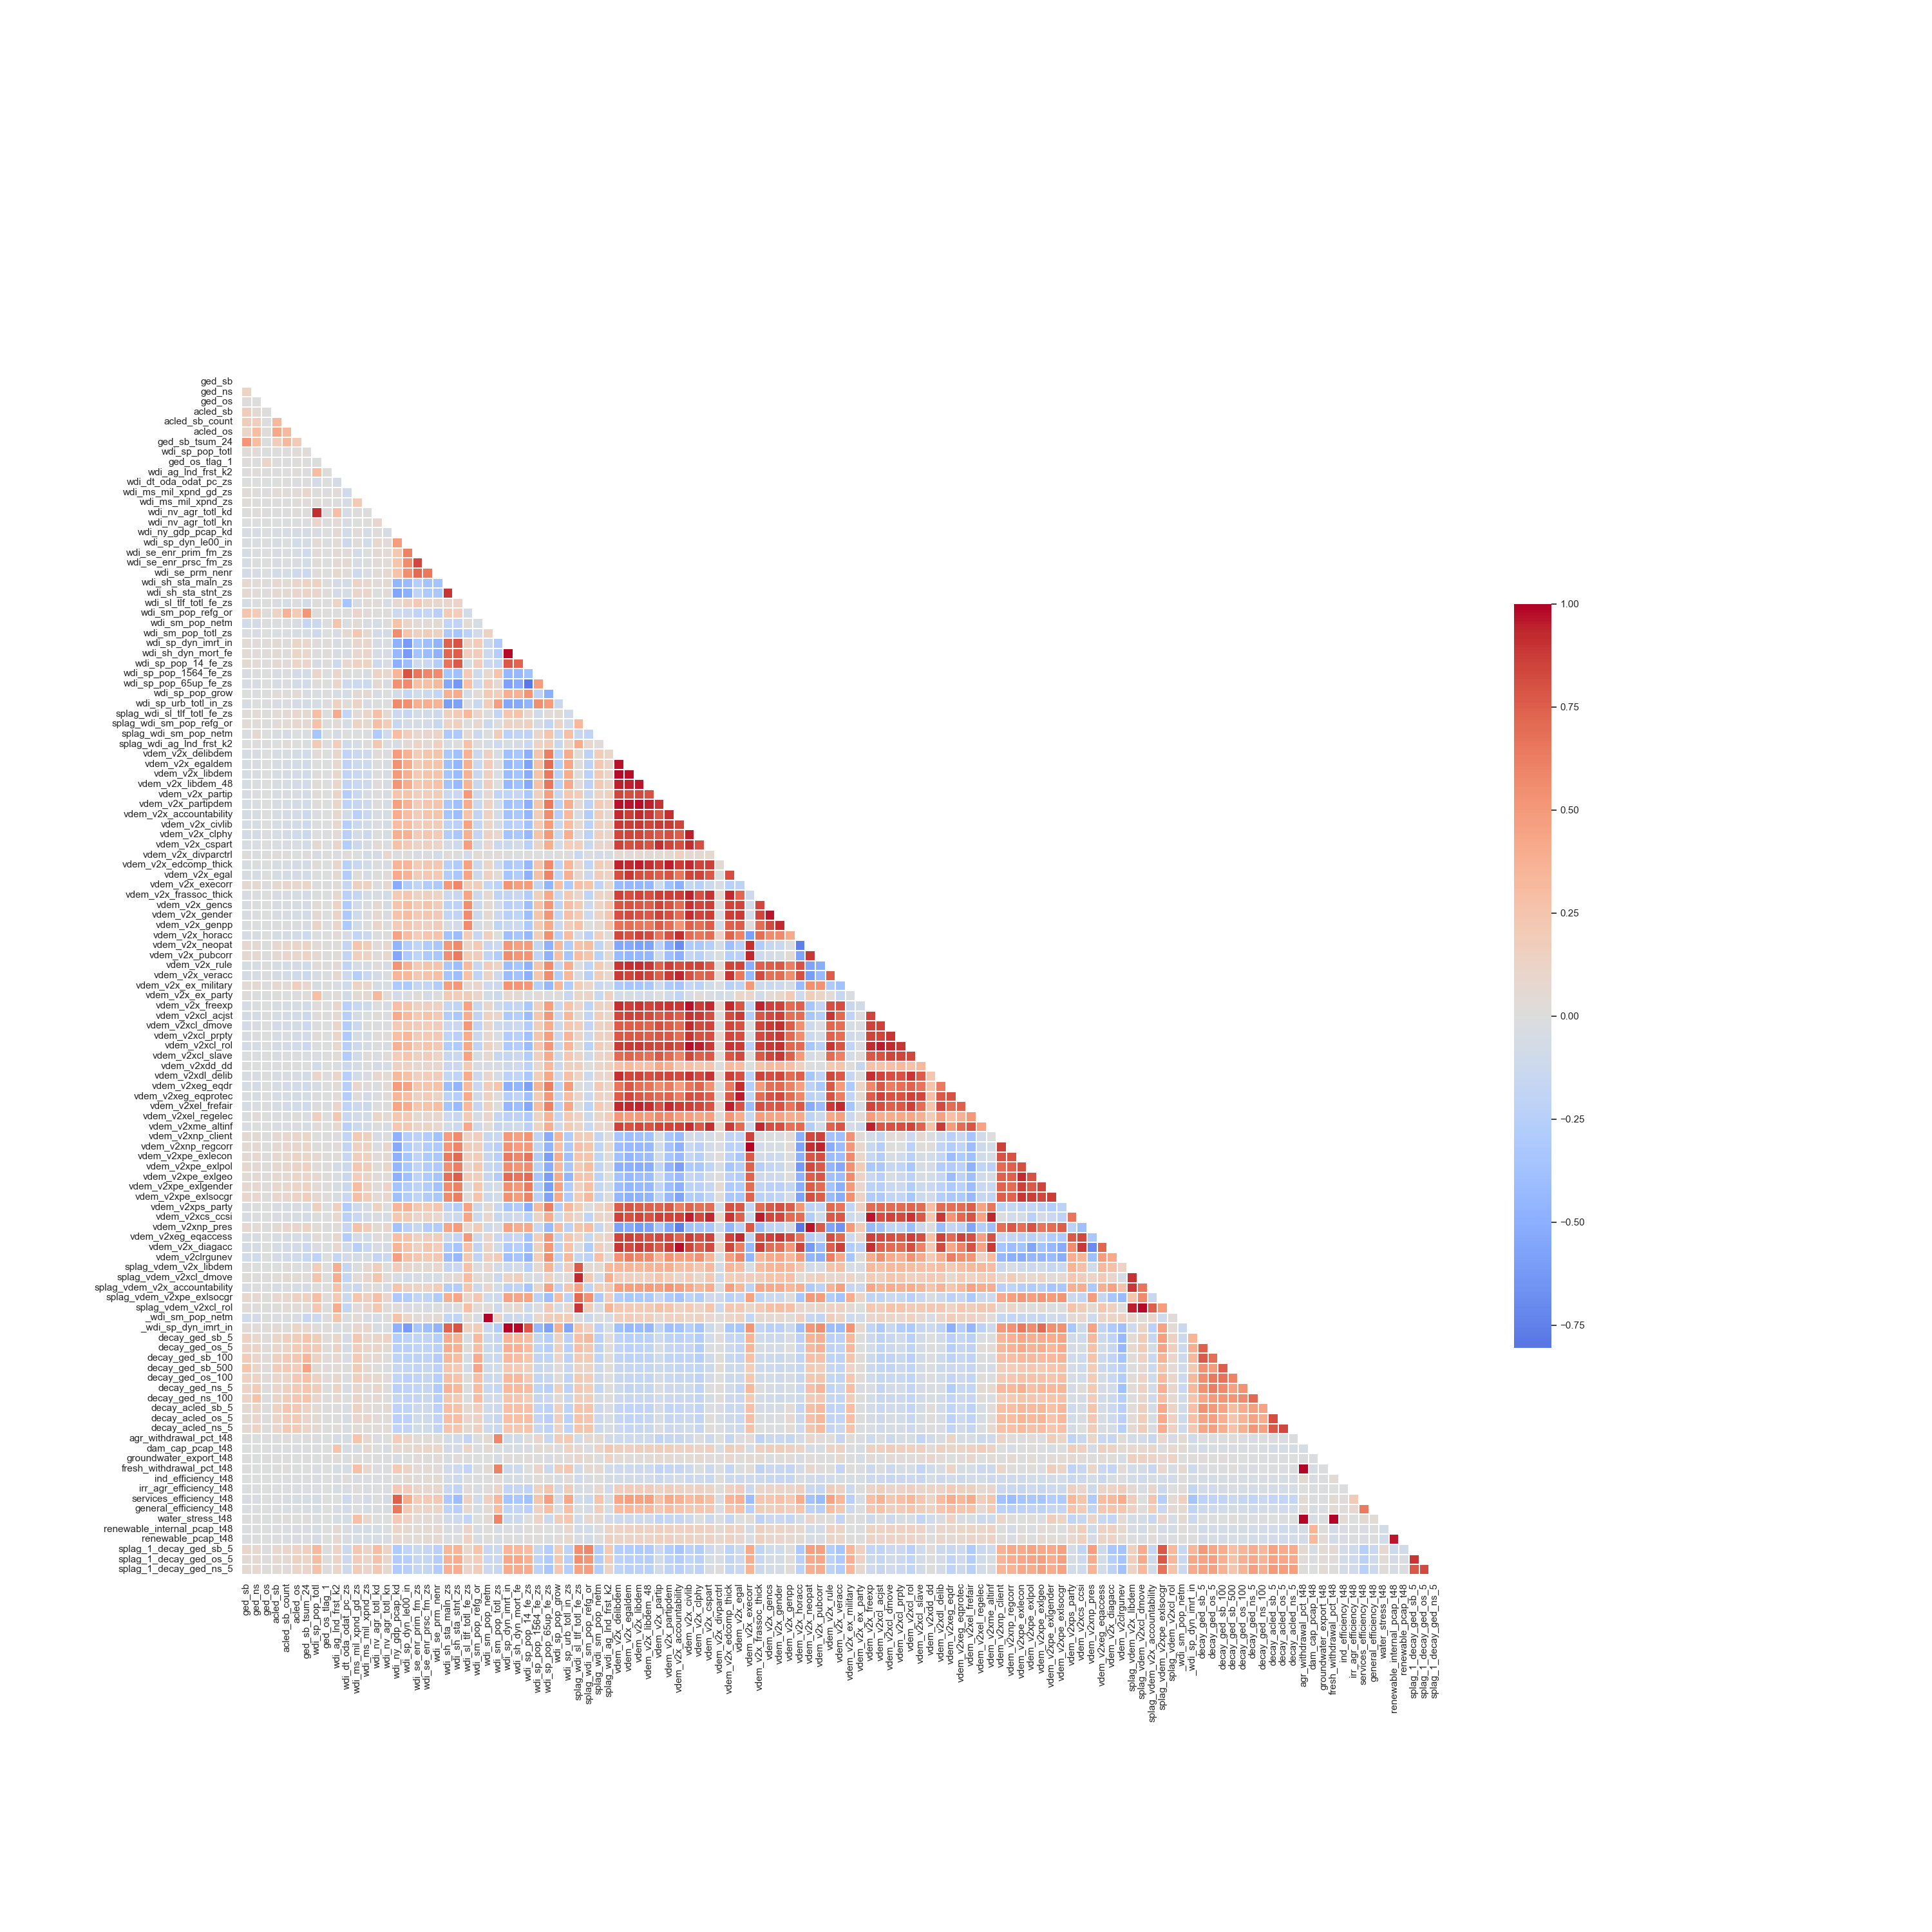
\includegraphics[width=\textwidth]{Figures/correlation_matrix.png}
        \centering
        \caption{Correlation matrix for original ViEWS competition dataset}
    \end{figure}


% Please note that the first paragraph of a section or subsection is
% not indented. The first paragraph that follows a table, figure,
% equation etc. does not need an indent, either.

% Subsequent paragraphs, however, are indented.

% \subsubsection{Sample Heading (Third Level)} Only two levels of
% headings should be numbered. Lower level headings remain unnumbered;
% they are formatted as run-in headings.

% \paragraph{Sample Heading (Fourth Level)}
% The contribution should contain no more than four levels of
% headings. Table~\ref{tab1} gives a summary of all heading levels.

% \begin{table}
% \caption{Table captions should be placed above the
% tables.}\label{tab1}
% \begin{tabular}{|l|l|l|}
% \hline
% Heading level &  Example & Font size and style\\
% \hline
% Title (centered) &  {\Large\bfseries Lecture Notes} & 14 point, bold\\
% 1st-level heading &  {\large\bfseries 1 Introduction} & 12 point, bold\\
% 2nd-level heading & {\bfseries 2.1 Printing Area} & 10 point, bold\\
% 3rd-level heading & {\bfseries Run-in Heading in Bold.} Text follows & 10 point, bold\\
% 4th-level heading & {\itshape Lowest Level Heading.} Text follows & 10 point, italic\\
% \hline
% \end{tabular}
% \end{table}


% \noindent Displayed equations are centered and set on a separate
% line.
% \begin{equation}
% x + y = z
% \end{equation}
% Please try to avoid rasterized images for line-art diagrams and
% schemas. Whenever possible, use vector graphics instead (see
% Fig.~\ref{fig1}).

% \begin{figure}
% \includegraphics[width=\textwidth]{fig1.eps}
% \caption{A figure caption is always placed below the illustration.
% Please note that short captions are centered, while long ones are
% justified by the macro package automatically.} \label{fig1}
% \end{figure}

%
% the environments 'definition', 'lemma', 'proposition', 'corollary',
% 'remark', and 'example' are defined in the LLNCS documentclass as well.
%

% For citations of references, use:
% In \cite{einstein} Einstein....

% In \cite{knuthwebsite} the authors

% This \cite{latexcompanion} is Latex.
%
% ---- Bibliography ----
%
% BibTeX users should specify bibliography style 'splncs04'.
% References will then be sorted and formatted in the correct style.
%
% \bibliographystyle{refs-style}
    \bibliographystyle{apacite}
    \bibliography{refs}
%
\end{document}
